
\chapter{Arquitetura}
\label{sec:arquitetura}

A arquitectura é uma etapa fundamental em todos os projecto porque é aqui que se define a estrutura e comportamento do sistema na sua globalidade e nas diferentes componentes.

Neste capítulo está exposta a arquitectura do 10.quest que servirá de \textit{guideline} para a implementação do projecto. Serão apresentadas diferentes prespectivas para analisar os diferentes aspectos do sistema. É de notar que as componentes a desenvolver pela restante equipa de desenvolvimento não será analisada e apenas será apresentada de forma superficial para fazer a ligação às componentes a desenvolver no ambito do estágio curricular.
Este capítulo é também uma exposição das decisões arquitecturais efectuadas no primeiro semestre, respeitando as restrições técnicas e de negócios.

Por fim será feita uma analise dos riscos envolvidos no desenvolvimento do projecto, o seu impacto e probabilidade de ocurrência e o respectivo plano de mitigação




\section{Analise da Arquitectura}
\label{analisearq}

Na analise da arquitectura serão apresentadas as restrições do projecto, que têm um impacto directo nas decisões de arquitectura, as diferentes prespectivas de arquitetura e as técnologias utilizadas.

\subsection{Restrições Técnicas}
As restrições técnicas são decisões técnicas arquiteturais que devem ser satisfeitas. O Sistema a desenvolver deve respeitar as seguintes restrições:

\textbf{Identificador: RT01}
\newline
\textbf{Título:} Arquitectura REST
\newline
\textbf{Descrição:} A comunicação entre a plataforma a desenvolver e o TCG deve seguir uma arquitectura REST.

\textbf{Identificador: RT02}
\newline
\textbf{Título:} Base de Dados
\newline
\textbf{Descrição:} Os dados utilizados pela aplicação devem ser guardados numa base de dados, visto tratar-se de um grande volume de dados que tem de permanecer organizado. Relativamente aos dados do TCG foi imposto que os dados não sejam duplicados e que esta informação seja acedida através de pedidos\acrshort{https}/\acrshort{rest}. PostegreSQL\cite{sql} é a base de dados relacional utilizada pela empresa e portanto será também utilizada no desenvolvimento deste projecto.

\textbf{Identificador: RT03}
\newline
\textbf{Título:} Framework Django\cite{django}
\newline
\textbf{Descrição:} A Framework Django é a técnologia utilizada pela empresa para desenvolver aplicações \textit{web} e \textit{\acrshort{saas}}. O uso desta técnologia foi imposta pelo \textit{Product Owner}.

\textbf{Identificador: RT04}
\newline
\textbf{Título:} Plataforma Web
\newline
\textbf{Descrição:} Todas as funcionalidades do sistema devem estar disponíveis através da plataforma web.

\subsection{Restrições de Negócio}
Nesta secção estão descritas as restrições de negócio, que podem ser entendidas com barreiras que a organização deve lutar para executar a sua estratégia. Estas restrições seguintes foram impostas pelo \textit{Product Owner} e devem ser satisfeitas na arquitectura do sistema:

\textbf{Identificador: RN01}
\newline
\textbf{Título:} Programa de Desenvolvimento
\newline
\textbf{Descrição:} O produto deve estar concluido e validado até dia 15 de Junho.



\subsection{\acrfull{mvc}}

A estrutura de um projeto Django é muitas vezes descrito como um projeto \acrshort{mvc}. Como podemos ver na Figura \ref{fig:arq-mvc}, o modelo \acrshort{mvc} é uma arquitectura de sowftare que separa a aplicação em três componentes lógicos principais. Por outras palavras este modelo separa a apresentação dos dados, da lógica que trata das \textit{interfaces} do utilizador, facilitando a programação das diferentes funcionalidades, \textit{debugging} e os testes das mesmas.

\begin{figure}[ht!]
	\begin{center}
		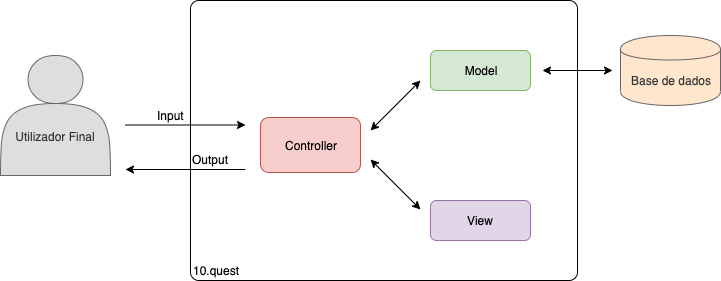
\includegraphics[width=1\textwidth]{img/arq/diagrama-MVC}
		\caption{Estrutura do Sistema}
		\label{fig:arq-mvc}
	\end{center}
\end{figure}

O componente \textbf{Model} controla a organização e armazenamento dos dados. Este módulo representa os dados que são transferidos entre os componentes Controller e View mas não representa nenhuma lógica no que diz respeito ao que é representado na camada de apresentação.

O componente \textbf{View} pode ser considerada a camada de apresentação. Este componente contém todas os ingredientes que constituem as interfaces do utilizador e controla a forma como a informação lhe é apresentada. Este modelo sabe como aceder ao modelo de dados que é apresentado ao utilizador contudo não sabe como o manipular nem o que significa.

Por último temos o componente \textbf{Controller}.  Este componente atua entre os modelos View e Model reagindo a eventos na View e respondendo a estes pedidos manipulando os dados utilizando o componente Model e interagindo com o componente View para renderizar o \textit{output}.


\subsection{Modelo C4}

Nesta secção encontra-se representada e descrita toda a arquitetura da plataforma 10.quest,  influênciada pelos objetivos de negócio, \textit{stakeholders}, requisitos e restrições técnica e de negócio, apresentados anteriormente.

Foram utilizados três diagramas para representar a arquitectura do sistema, utilizando o \textbf{modelo C4}\cite{c4}: diagrama de contexto, diagrama de contentores, diagrama de componentes e o diagrama de classes.

Os diferentes diagramas representam diferentes perspectivas e níveis de abstração e foram feitos com o intuito de facilitar a compreensão da arquitetura permitindo à equipa de desenvolvimento visualizar os diferentes níveis de granularidade. 

O diagrama de contexto mostra a relação entre o sistema que vai ser desenvolvido e outros agentes como por exemplo utilizadores e sistemas externos.  Este é o diagrama com maior nível de abstração e é bom para sublinhar as dependencias externas que a equipa de desenvolvimento tem que integrar no sistema. 

O diagrama de contentores apresenta um maior detalhe (i. e. relativamente ao diagrama de contexto) e motras os diferentes contentores que constituem o sistema (e. g. bases de dados, aplicações, microserviços etc...). Neste diagrama são também definidas algumas decisões arquitecturais. 

Por último temo o diagrama de componentes aproxima um contentor individualmente e mostra todos os componentes que constituem esse contentor. Desta forma conseguimos perceber as principais funcionalidades do sistema. 


\subsubsection{Diagrama de Contexto}

Como foi referido no Catípulo \ref{sec:introducao} o 10.quest é uma plataforma de inbound marketing que consiste num \textit{backoffice} para criação de questionários, concursos e criação de formulário com o auxilio do \acrshort{tcg}.

Como podemos ver na Figura \ref{fig:arq-contexto} o 10.quest interage com seis sistemas externos. O SendGrid\cite{sg} é um \acrshort{saas}, na \textit{cloud}, que fornece um serviço de entrega de emails. Este serviço permite enviar emails através de APIs flexíveis garantindo uma disponibilidade  de 99.999\% \cite{sguptime}. 
O TCG, tal como foi referido no Capítulo \ref{sec:estado-arte}, é uma plataforma de criação de formações que tem como principal objectivo transformar PDFs numa aprendizagem baseada em tentativa erro. Algumas das funcionalidades do \acrshort{tcg} serão utilizadas pelo 10.quest.
Para partilhar os questionários, concursos e formações o 10.quest irá utilizar as APIs do Facebook, LinkedIn, Twitter e Instagram.


\newpage

\begin{figure}[ht!]
	\begin{center}
		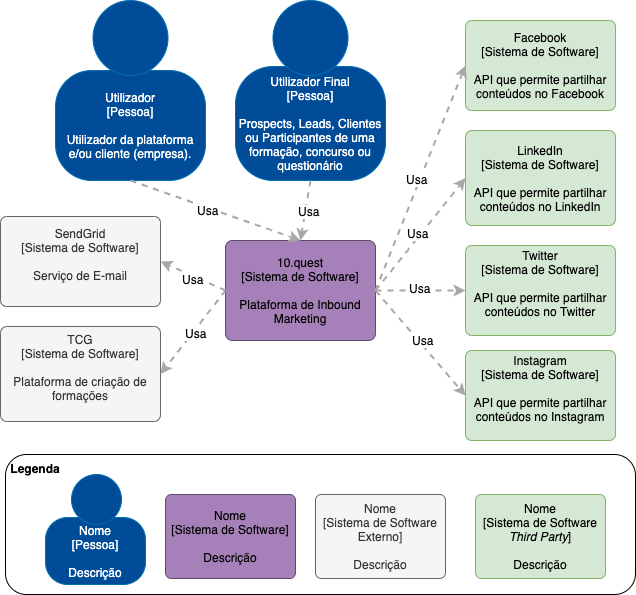
\includegraphics[width=0.9\textwidth]{img/arq/diagrama-contexto}
		\caption{Diagrama de Contexto}
		\label{fig:arq-contexto}
	\end{center}
\end{figure}

\subsubsection{Diagrama de Contentores}

Na Figura \ref{fig:arq-contentores} está representado o diagrama de contentores, onde se pode observar com mais detalhe a constiuição do sistema de software.

Os utilizadores podem ser de dois tipos: o utilizador do backoffice que tem acesso a todas as funcionalidade da plataforma e o utilizador final que tem acesso a uma página web para participar nas formações, concursos e ou questionários.

A aplicação web efectua os pedidos dos utilizadores, através de pedidos \acrshort{https}/\acrshort{rest} à API. A aplicação web será a camada de apresentação da API e ambos serão desenvolvidos em Django. A API será o contentor responsável por tratar de todos os pedidos efectuados pelos utilizadores do \textit{backoffice}. Para este efeito a API implementa um conjundo de funcionalidades, representadas na Figura \ref{fig:arq-componentes1}, que manipulam um conjunto de dados armazenados numa base de dados relacional PostgreSQL, para conseguir as informações necessárias.
\newpage

\begin{figure}[ht!]
	\begin{center}
		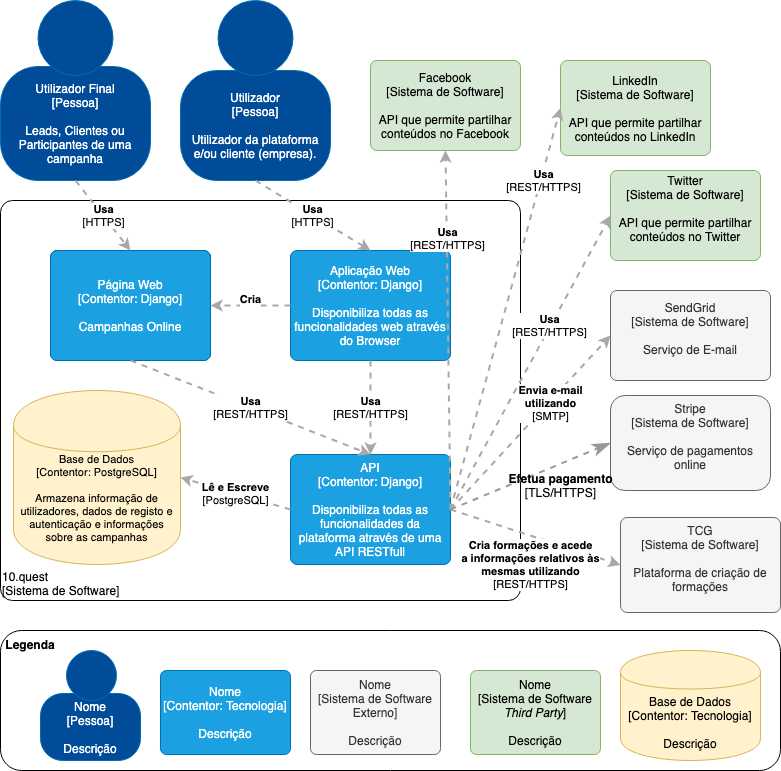
\includegraphics[width=0.9\textwidth]{img/arq/diagrama-contentores}
		\caption{Diagrama de Contentores}
		\label{fig:arq-contentores}
	\end{center}
\end{figure}

\subsubsection{Diagrama de Componentes}

Na Figura \ref{fig:arq-componentes} é apresentado o diagrama de componentes e na Figura \ref{fig:arq-componentes1} são as presentados os componentes da API. 

A autenticação é necessária para que os pedidos sejam aceites e mapeados pela API. Para isto a componente "Autenticação", permite ao utilizador efetuar a sua autenticação e verifica a autenticidade do mesmo, em cada pedido, através de tokens. Desta forma, caso o utilizador esteja autenticado os seus pedidos \acrshort{https}/\acrshort{rest} avançam para a componente API , que inclui todas as componente (i. e. funcionalidades) que dão resposta aos requisitos funcionais definidos para o projeto.

A componente "Dados" permite às restantes componentes interagir com a base de dados, tanto para ler, como para escrever.


\begin{figure}[ht!]
	\begin{center}
		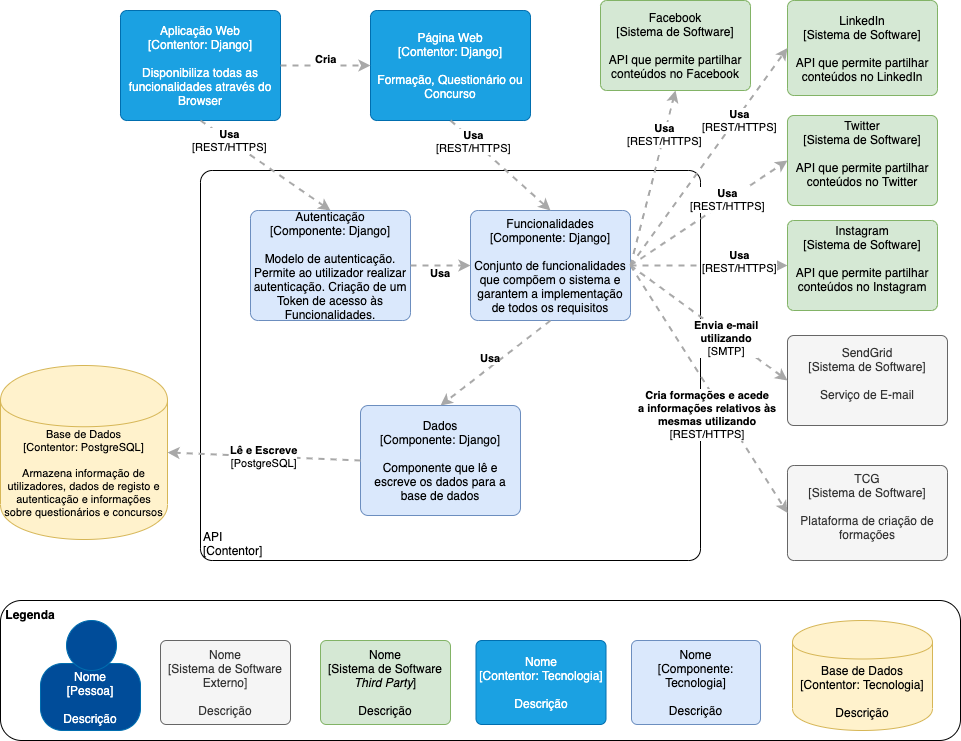
\includegraphics[width=0.86\textwidth]{img/arq/diagrama-componentes}
		\caption{Diagrama de Componentes}
		\label{fig:arq-componentes}
	\end{center}
\end{figure}

\begin{figure}[ht!]
	\begin{center}
		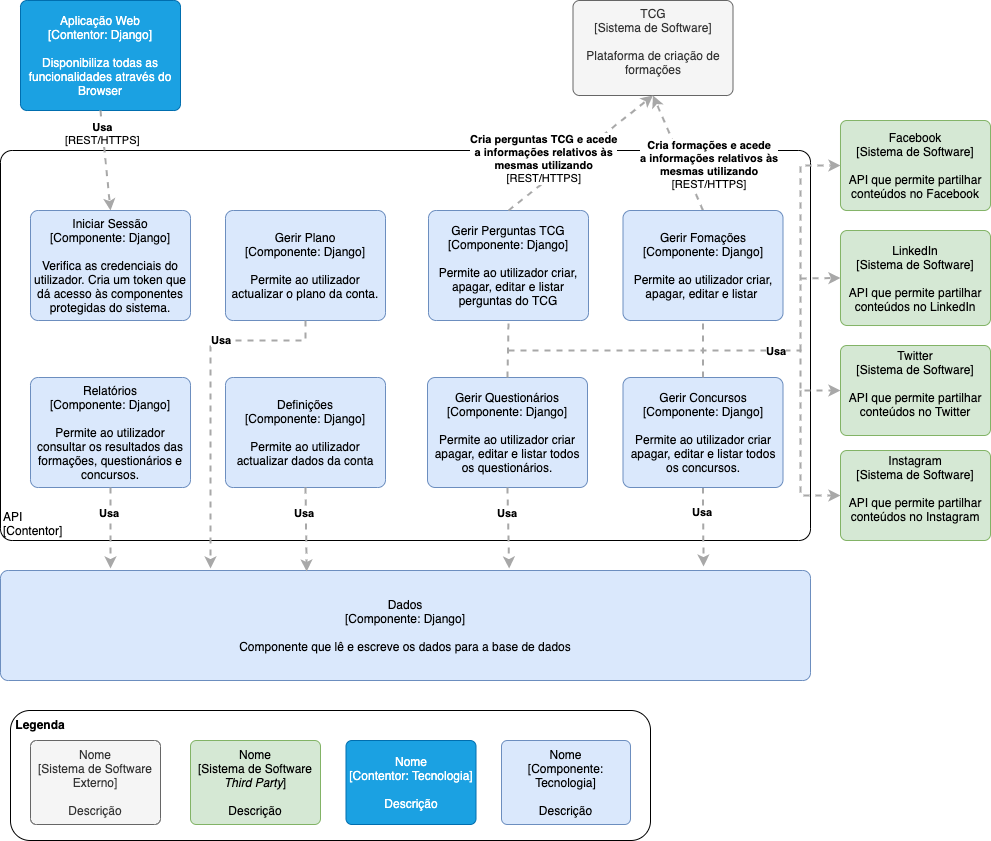
\includegraphics[width=0.87\textwidth]{img/arq/diagrama-componentes1}
		\caption{Diagrama Componentes da componente Funcionalidades}
		\label{fig:arq-componentes1}
	\end{center}
\end{figure}

\newpage

%\subsection{Modelo Sequencial}

%\subsection{Modelo de Dados}


%  FALTA CAPITULO PARA DISCUSSÂO VALIDAÇÂO DA ARQUITECTURA. Escrever assim que todas as decisões estiveres feitas

\subsection{Técnologias Utilizadas}

Grande parte das técnologias ainda estão por definir.

\section{Analise de Riscos}
\label{analiseriscos}

Antes de se inicializar a fase de desenvolvimento do projeto é importante realizar uma analise aos possíveis riscos associados ao projeto. Desta forma é importante antecipar/identificar os diferentes riscos que contribuem para o insucesso do projeto para que se possam criar estratégias de mitigação de maneira a minizar o impacto de cada risco. Os diferetes riscos serão classificados tendo em conta o seu impacto e a sua probabilidade.

\begin{itemize}
	\item[--] \textbf{Probabilidade}
		\subitem \textbf{Baixa}: Menor que 30\%
		\subitem \textbf{Média}: Entre 30\% a 70\%
		\subitem \textbf{Alta}: Superior a 70\%
	\item[--] \textbf{Impacto}
		\subitem \textbf{Baixo}: Interfere no desenvolvimento do projecto.
		\subitem \textbf{Médio}: Interfere no desenvolvimento do projecto e força alterações no produto final.
		\subitem \textbf{Alto}: Compromete a finalização do projeto.
\end{itemize}

De seguida serão listados todos os riscos associados ao projeto e respectivo plano de mitigação para tentar reduzir o impacto do mesmo:

\textbf{R01 - Dependência de sistemas externos}
\begin{itemize}
	\item[--] \textbf{ID}: R01
	\item[--] \textbf{Descrição}: Não se pode garantir uma disponibilidade de 100\% em todos os sistemas externos (e. g. APIs offline) sendo que em algumas ocasiões o sistema pode ter algumas funcionalidades indisponíveis.
	\item[--] \textbf{Estratégia de Mitigação}: Quando um serviço externo está temporariamente indisponível, apesar algumas funcionalidades também indisponíveis, o sistema deve tratar os pedidos do utilizador de forma a afetar a experiencia do utilizador, ou no pior dos casos para reduzir o impacto no mesmo.
	\item[--] \textbf{Probabilidade}: Baixa
	\item[--] \textbf{Impacto}: Baixo
\end{itemize}

\textbf{R02 - Dificuldade em implementar o sistema de pagamento}
\begin{itemize}
	\item[--] \textbf{ID}: R02
	\item[--] \textbf{Descrição}: A falta de experiência por parte do aluno na implementação de métodos ou serviços de pagamentos põe em causa a boa implementação do mesmo e pode comprometer uma das principais funcionalidades do produto final.
	\item[--] \textbf{Estratégia de Mitigação}: Deve ser feita uma análise cuidada dos métodos ou serviços de pagamentos disponíveis para integrar com a técnologia de desenvolvimento da plataforma e de seguida deve ser lida a documentação com atenção para garantir uma boa implementação da mesma.
	\item[--] \textbf{Probabilidade}: Alta
	\item[--] \textbf{Impacto}: Alto
\end{itemize}

\textbf{R03 - Adaptação a novas tecnologias }
\begin{itemize}
	\item[--] \textbf{ID}: R03
	\item[--] \textbf{Descrição}: A não familiarização, por parte do aluno, com as principais técnologias que irão ser utilizadas na desenvolvimento do projeto, pode criar atrasos implementaçãodevido à fala de experiância e/ou substimação do tempo definido para cada tarefa, comprometendo a implementação de algumas funcionalidades.
	\item[--] \textbf{Estratégia de Mitigação}: Para além das horas definidas no planeamento do projecto, o aluno terá ed dispensar horas extra de modo a conseguir concluir a implementação e validação de todas as funcionalidades.
	\item[--] \textbf{Probabilidade}: Média
	\item[--] \textbf{Impacto}: Médio
\end{itemize}

\textbf{R04 - Novo requisito funcional}
\begin{itemize}
	\item[--] \textbf{ID}: R04
	\item[--] \textbf{Descrição}: As necessidades do cliente podem mudar com o tempo e nesse sentido é possível o aparecimento de um novo requisito funcional.
	\item[--] \textbf{Estratégia de Mitigação}: Reavaliação do plano de desenvolvimento e reestruturação de algumas funcionalidades para que fiquem mais genéricas e assim possa haver tempo para a realização do(s) novo(s) requisito(s). Em alternativa poderão também ter que ser dispensadas algumas horas pelo aluno de modo a cumprir com o plano de desenvolvimento.
	\item[--] \textbf{Probabilidade}: Baixa 
	\item[--] \textbf{Impacto}: Médio
\end{itemize}

Para uma melhor compreensão e visualização dos riscos associados ao projecto será apresentado de seguida, na Tabela \ref{tab:riscos}, um resumo da probabilidade e o impacto de cada risco.

\begin{table}
	\centering
\begin{tabular}{ | l | l | l | l |}
	\hline
	\tikz{\node[below left, inner sep=1pt] (def) {Probabilidade};%
		\node[above right,inner sep=1pt] (abc) {Impacto};%
		\draw (def.north west|-abc.north west) -- (def.south east-|abc.south east);}
	& Baixo & Médio & Alto\\
	\hline
	Baixa & \cellcolor{green}\centering R01 & \cellcolor{yellow}R04& \cellcolor{orange}\\
	\hline
	Média & \cellcolor{yellow} & \cellcolor{orange}R03 & \cellcolor{darkOrange}\\
	\hline
	Alta & \cellcolor{orange} & \cellcolor{darkOrange} & \cellcolor{red}R02\\
	\hline
\end{tabular}
\begin{center}
\caption {Classificação dos riscos associados ao projecto}
\label {tab:riscos}
\end{center}
\end{table}



% Listar os Riscos em que activei a estratégia de mitigação e de seguida voltar a mostrar a tabela actualizada







%-------------------------------------------------------------------------------------------------
\blankpage
%-------------------------------------------------------------------------------------------------

\glsresetall
